\chapter{Knowledge}
\label{chapter:knowledge}
In order to clearly understand the Hawkes process, we will introduce the definition of point process, counting process and conditional intensity function. And then we discuss the  inhomogeneous Poisson process. It is necessary to discuss because one can view the Hawkes process as a generalization of the (time) inhomogeneous Poisson process.
\section{Point process and counting process}
\begin{definition}
	\cite{hawkes} \textbf{(Point process)} Let $\{T_i, i \in \mathbb{N} \}$ be a sequence of non-negative random variables such that $\forall i \in \mathbb{N}, T_i<T_{i+1}$. Then $\{T_i, i \in \mathbb{N} \}$ is a (simple) point process.
\end{definition}
\begin{definition}
	\cite{hawkes} \textbf{(Counting process)} A counting process is a stochastic process $(N(t):t \geq 0)$ taking values in $\mathbb{N}_0$ that satisfies $N(0)=0$, is almost surely finite, and is a right-continuous step function with increments of size +1. Denote by $(\mathcal{H}(u): u \geq 0)$ the history of the arrivals up to time $u$.
\end{definition}
\noindent
For example:
\begin{itemize}
	\item If $N(t)$ is the number of persons who enter a store by time $t$, then $(N(t):t \geq 0)$ is a counting process in which an event corresponds to a person enters the store.
	\item If $N(t)$ is the number of goals that a given football player scores by time $t$ , then $(N(t):t \geq 0)$ is a counting process in which an event of the process will occur whenever the football player scores a goal.
\end{itemize}
\begin{figure}[H]
	\centering
	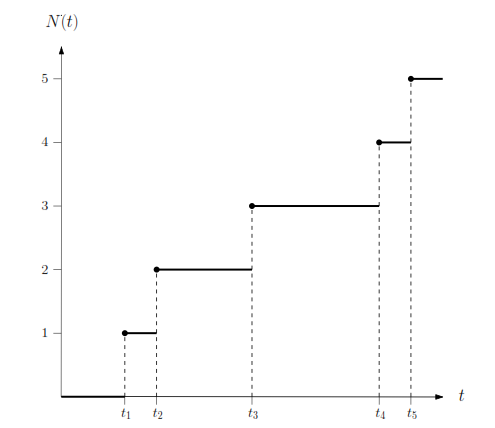
\includegraphics{coutingprocess}
	\caption[Point process $\{t_1, t_2,...\}$ and corresponding counting process $N(t)$.]{Point process $\{t_1, t_2,...\}$ and corresponding counting process $N(t)$.}
\end{figure}
\section{Conditional intensity function}
It is difficult to work with the conditional arrival distribution $f^*(t)$, so one used another characterization of point process which was called conditional intensity function. This function is defined in the form
\begin{align*}
	\lambda^*(t)=\dfrac{f^*(t)}{1-F^*(t)}
\end{align*}
where $f^*(t)$ is the conditional probability density function (p.d.f) of the next arrival given the previous arrival history and $F^*(t)$ is the cumulative distribution function (c.d.f) of the next arrival given the previous arrival history.
\begin{definition}
	\label{def:cif}
	\cite{hawkes} \textbf{(Conditional intensity function)} Consider a counting process $N(.)$ with associated histories $\mathcal{H(.)}$. If a function $\lambda^*(t)$ exists such that
	\begin{align*}
		\lambda^*(t) = \lim_{h\downarrow 0} \frac{\mathbb{E}[N(t + h) - N(t)|\mathcal{H}(t)]}{h}
	\end{align*}
	which only relies on information of $N(.)$  in the past (that is, $\lambda^*(t)$ is $\mathcal{H}(t)$ - measurable), then it is called the conditional intensity function of $N(.)$.
\end{definition}
\begin{figure}[H]
	\centering
	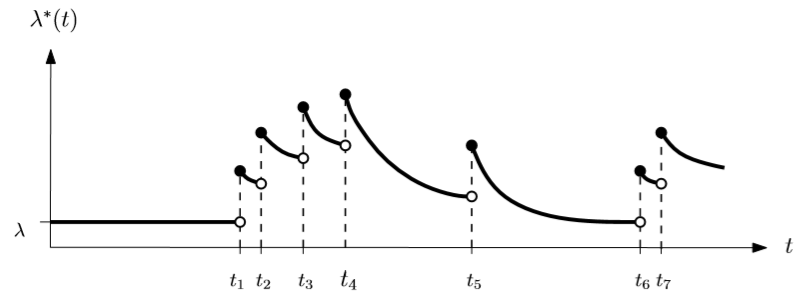
\includegraphics[scale=.75]{conditionintensityfunction}
	\caption[The conditional intensity function for a self-exciting process.]{The conditional intensity function for a self-exciting process.}
\end{figure}
\section{Inhomogeneous Poisson process}
\subsection{Description}
The inhomogeneous Poisson process is a generalization of the homogeneous Poisson process that intensity function depends on the time $t$.
\begin{definition}
	\textbf{(Inhomogeneous Poisson Process)} Consider $(N(t):t \geq 0)$ a counting process, that satisfies
	\begin{align*}
	\mathbb{P}(N(t+h)-N(t)=m|N(t))=
	\begin{cases}
	\lambda(t)h,& \text{if } m=1\\
	o(h) ,& \text{if } m>1\\
	1-\lambda(t)h+o(h),& \text{if } m=0
	\end{cases}
	\end{align*}
	Then a counting process $N(t)$ is called an inhomogeneous Poisson process with an intensity function $\lambda:\mathbb{R}^+ \rightarrow \mathbb{R}^+$.
\end{definition}
The intensity function $\lambda(t)$ of an inhomogeneous Poisson process is a deterministic function.
\begin{definition} \cite{thesis} \textbf{(Mean Value Function)} The function 
	\begin{align*}
	m(t) = \int_{0}^{t} \lambda(y)dy
	\end{align*}
	is called the mean value function of the inhomogeneous Poisson process.
\end{definition}
\begin{theorem}
	\cite{thesis} If $\{ N(t), t \geq 0\}$ is a non-stationary Poisson process with intensity function $\lambda(t), t \geq 0$, then $N(t + h) - N(h
	)$ is a Poisson random variable with mean $m(t + h) - m(h) = \displaystyle\int_{h}^{h + t}\lambda(y)dy$.
\end{theorem}
\subsection{The algorithm}
The idea of this algorithm is to generate a homogeneous Poisson process, and then remove the points probabilistically so that the remaining points satisfy the time-varying intensity $\lambda(.)$. This algorithm requires the conditional intensity to be upper bounded, i.e., $\exists M$ such that $\lambda(.) \leq M$ on $[0,T]$.
\begin{breakablealgorithm}
	\caption{Generate an inhomogeneous Poisson process by thinning.}
	\label{algorithm:poison}
	\begin{algorithmic}[H]
		\noindent
		\algorithmicrequire{ $T$ is the time to simulate; \\
			\hspace*{1.8 cm}$\lambda(.)$ is the intensity function; \\
			\hspace*{1.7 cm}$M$ is upper bounded value;}\\
		\algorithmicensure{ Retrieve the simulated process $\{t_1, t_2,...,t_n\}$ on $[0,T]$;}\\
%		\algorithmicensure{ The vector $P$ containing the times of occurrences $\{t_1, t_2,...,t_n\}$;}\\
		\textbf{Require:} $\lambda(.) \leq M$ on $[0,T]$.\\
		\begin{itemize}
			\item [1.] $P\leftarrow []$, $t\leftarrow0$
			\item [2.] \textbf{while} $t<T$ \textbf{do}
			\item [3.] \hspace*{.6cm}Generate next candidate point: $E \leftarrow$ Exp $(M)$,  $t \leftarrow t+E$
			\item [4.] \hspace*{.5cm} Keep it with some probability:  $U \leftarrow$ Unif$(0,M)$
			\item [5.] \hspace*{.55cm} \textbf{if} $t <T$ \textbf{and} $U \leq \lambda(t)$ \textbf{then}
			\item [6.]  \hspace*{1.2cm}$P \leftarrow [P,t]$
			\item [7.] \hspace*{.65cm}\textbf{end if}
			\item [8.] \textbf{end while}
		\end{itemize}
	\end{algorithmic} 
\end{breakablealgorithm}

